\section{Shield vibrations}


\begin{figure}[!htbp]
  \centering
  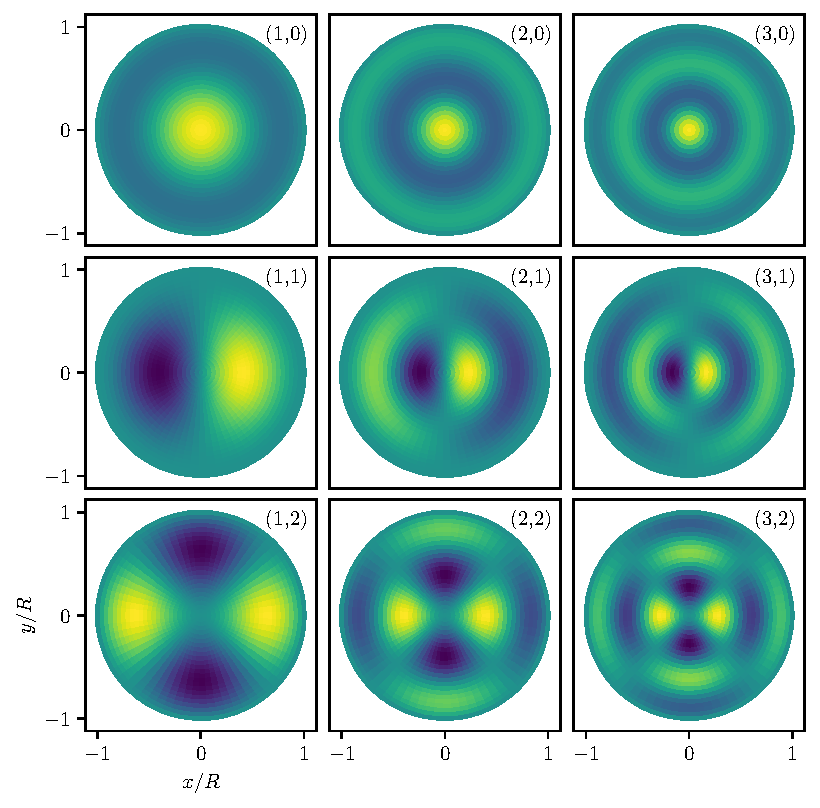
\includegraphics[width=\textwidth]{./../figures/vibrations/vibrational-modes.pdf}
  \label{fig:4:vibrational-modes}
  \caption{Vibrational modes of a spherical plate fixed at the edge with $R/d = 1000$.}
\end{figure}


The modes $(k,l),\, 1 \leq k, \, 0 \leq l$ have the shape
\begin{equation}
  u_{kl}(r, \theta, t) = A\left[J_l(\sqrt{\beta_k}r) - \frac{J_l(\sqrt{\beta_k}r_s)}{I_l(\sqrt{\beta_k}r_s)}I_l(\sqrt{\beta_k}r)\right]\cos(l\theta+\phi_1)\sin(\omega_{kl}t+\phi_2)
\end{equation}
with
\begin{equation}
  \beta_k = \frac{\tilde{r}_k^2}{r_s^2} \quad \quad \omega_{kl} = \frac{\tilde{r}_k^2}{r_s^2}\sqrt{\frac{D}{\rho d}} = \tilde{x}_l^2\frac{d}{r_s^2}\sqrt{\frac{E}{12\rho(1-\nu^2)}} ,
\end{equation}
where $\tilde{r}_k$ is the $k$-th solution of the equation
\begin{equation}
  J_l(\tilde{r}_k)I_{l+1}(\tilde{r}_k)+I_l(\tilde{r}_k)J_{l+1}(\tilde{r}_k) = 0 .
\end{equation}


\subsection{Occupation of the vibration-modes}
Because of the modes $u_{kl}$, both superposition states of delocalized cat-state in front of the shield are effected by a slightly different Casimir-force. This force depends on the surface-to-surface distance $\mathscr{L}$ between the shield and the mass.
This distance changes slightly due to the thermal motion of the shield by a difference of $A \cdot u_{k,l}(r_\mathrm{pos})$ where $r_\mathrm{pos}$ is the position of the particle. 
During time evolution, a slightly different phase is introduced for the two delocalized states. 
I am interested, which modes matters the most and introduce the most dephasing in a parallel superposition in front of the shield. This information is useful for a worst-case estimate on how much angular and distance fluctuations in the positioning of the particle are introduced through thermal effects. 
Experimentally, one therefore needs to find a regime in which entanglement can still be measured regardless of these thermal vibrations.

Assuming a shield made out of copper with $\rho = 8960\si{kg/m^3}$, $E = 110\si{GPa}$ and $\nu = 1/3$, the vibrational frequencies for a thin shield ($d = 100\si{nm}$ and $r_s = 0.01\si{m}$) are given in the order of $\omega_{1,0}=11.0\si{s^{-1}}$ up to $\omega_{10,11} = 3108.9\si{s^{-1}}$.
Because of these low frequencies, the energy $\hbar \omega$ of the mode vibrations are much smaller than the thermal energy $k_B T$ for a reasonable temperature. This means, that all modes are approximately occupied uniformly.
The amplitude $z$ of each mode of the plate vibrations can be thought of as an quantum harmonic oscillator with frequency $\omega_{kl}$. At a temperature $T$, the expected amplitude is given by $\avg{z_{kl}} = 0$ with a variance of (a derivation is given in appendix \ref{apx:thermal-harmonic-oscillator})
\begin{equation}\label{eq:4:amplitude-variance}
  \avg{z_{kl}^2}_T = \frac{\hbar}{2\tilde{m}\omega_{kl}}\coth(\frac{\hbar \omega_{kl}}{2k_BT}) \approx \frac{k_B T}{\tilde{m}\omega_{kl}^2}
\end{equation}
where in the last step $\hbar\omega \ll k_B T$ was used. $\tilde{m}$ is the \textit{effective mass} of the mode in which the precise shape is considered. A intuitive estimation for this mass can be given by the average of the mode 
\begin{equation}\label{eq:4:effective-mass}
  \tilde{m} = m\frac{1}{\pi r_s^2}\int_0^{r_s} \dd r \int_0^{2\pi} r\dd\theta \, u_{kl}(r, \theta, t) .
\end{equation}
with $m=\rho \pi r_s^2 d$ being the total mass of the shield.
Due to the high occupation number of oscillator modes, the probability $p(z)$ of finding an oscillation with amplitude $z$ is approximately a gaussian normal distribution around $\avg{z_{kl}} = 0$ with the standard deviation given by the square-root of $(\Delta z_{kl})_T^2 = \avg{z_{kl}^2}_T - \avg{z_{kl}}$.
Luckily it seems that the on average, the standard deviation decreases with $1/\omega$ which means, that higher-order modes with larger frequencies are still highly occupied but should contribute less to the total vibration.
To quantify this, I considered the dephasing of a single parallel delocalized cat-state in front of the plate. The phase difference $\Delta \phi$ is given by
\begin{equation}\label{eq:4:phase-difference}
  \Delta\phi(z) = \frac{t}{\hbar} \frac{\hbar c \pi^3}{720} R \left[\frac{1}{(\mathscr{L}-z \cdot u_{kl}(r- \Delta x/2))^2} - \frac{1}{(\mathscr{L}-z \cdot u_{kl}(r + \Delta x/2))^2} \right]
\end{equation}
when the particle is placed at a distance $r$ from the center of the plate. In the following the two cases are considered, where the particle is placed in the center at $r=0$ and in the worst-case position of mode $(1,0)$, where the gradient is maximized ($r \approx 0.5274 r_s$).
The dephasing rate $\gamma$ is now given by
\begin{equation}\label{eq:4:average-dephasing}
  e^{-\gamma} = \avg{e^{-i\Delta\phi}} = \int_{-\infty}^{\infty} \dd z \, \frac{1}{\sqrt{2 \pi (\Delta z_{kl})_T^2}} \exp{-\frac{z^2}{2 (\Delta z_{kl})_T^2}} e^{-i \Delta\phi(z)} .
\end{equation}
In \cref{fig:4:dephasing} the dephasing $\gamma$ is shown.
\begin{figure}[!htbp]
  \centering
  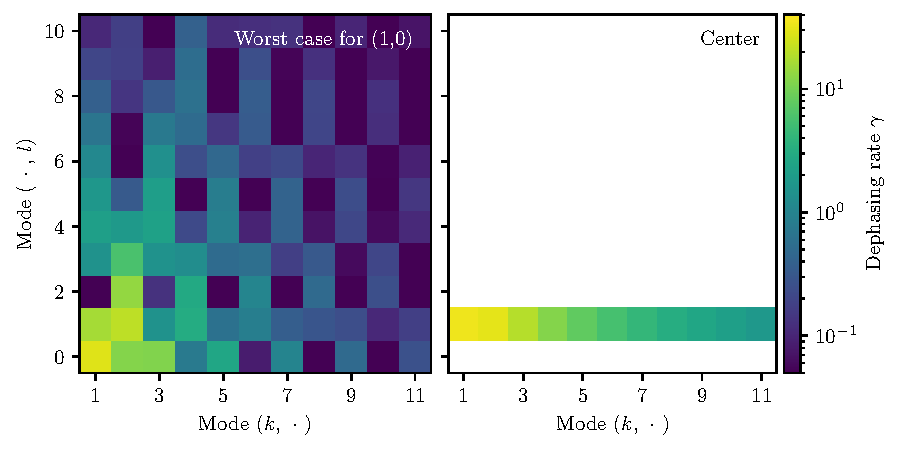
\includegraphics[width=\textwidth]{./../figures/vibrations/vibrational-dephasing-rate.pdf}
  \caption{Dephasing rate $\gamma$ of a delocalized cat-state positioned parallel to the shield at $T=4\si{K}$. \textbf{left:} the worst-case estimate where the state is placed in the point with the maximum gradient ($r\approx 0.5274 r_s$). \textbf{right:} realistic scenario with the cat-state placed at the center.}
  \label{fig:4:dephasing}
\end{figure}
The non-trivial behavior arises because of the different mode-shapes. Nevertheless, a clear trend is observable where all highly excited modes don't contribute to the dephasing.
Assuming, that the amplitude $z$ is much smaller than $\mathscr{L}$ \footnote{Which is true, considering that $\sqrt{(\Delta z_{1,0}^2)_T}\approx 1.807 \times 10^{-9}\si{m}$ compared to $\mathscr{L} \approx R \sim 10^{-6}\si{m}$.}, the phase-difference eq. \eqref{eq:4:phase-difference} can be expanded to
\begin{equation}
  \Delta\phi(z) \approx \frac{c \pi^3 R t}{720} \cdot \frac{2\left(u_{kl}(r - \Delta x/2) -u_{kl}(r + \Delta x/2)\right)z}{\mathscr{L}^3} \equiv g z
\end{equation}
Averaging over $z$ using again the probability distribution $p(z)$ like in eq. \eqref{eq:4:average-dephasing}, the resulting expression is given by
\begin{equation}
  e^{-\gamma} \approx \int_{-\infty}^{\infty} \dd z \, p(z) e^{-i g z} = \exp{-\frac{g^2 (\Delta z_{kl})^2_T}{2}} \approx \exp{-\frac{\Delta\phi^2\left(\sqrt{(\Delta z_{kl})^2_T}\right)}{2}} .
\end{equation}
It is therefore enough for further calculations, to actually use the thermal variance of the oscillator $(\Delta z_{kl})^2_T$ for the amplitude for all modes. The error done by this approximation is shown in \cref{fig:4:dephasing-approximation-error}.
\begin{figure}[!htbp]
  \centering
  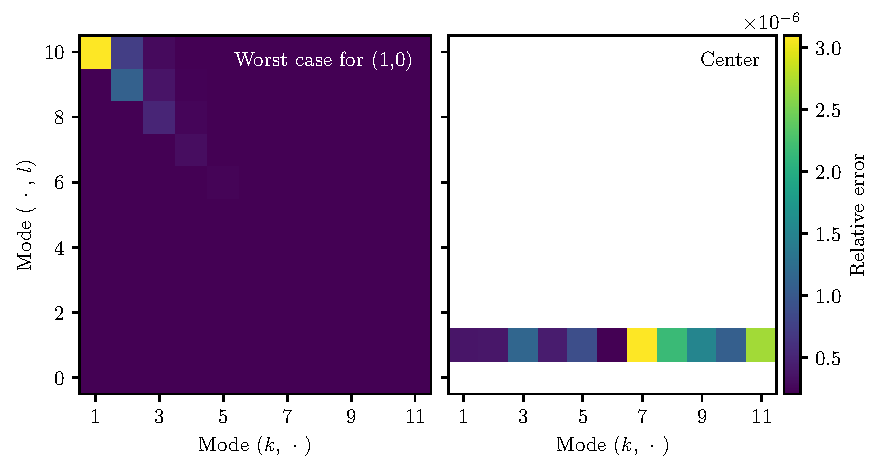
\includegraphics[width=\textwidth]{./../figures/vibrations/vibrational-dephasing-approximation-error.pdf}
  \caption{Relative error $\abs{\gamma_\mathrm{approx} / \gamma - 1}$ by using $\gamma_\mathrm{approx} = \Delta\phi^2\left(\sqrt{(\Delta z_{kl})^2_T}\right)/2$. Hardly any notable error is therefore made by these approximations for higher order modes. The approximation only overestimates the lowest modes by a factor of $\sim 3$.}
  \label{fig:4:dephasing-approximation-error}
\end{figure}
Furthermore, the numerical results in \cref{fig:4:dephasing} suggest that only very low modes need to be taken into account for all further considerations.

\subsection{The Hamiltonian}
\begin{equation}
  H = \hbar \omega \left(a^\dagger a + \frac{1}{2}\right) \otimes \mathbb{1} + f_A(\op{z})\otimes\ketbra{\psi_A} + f_B(\op{z})\otimes\ketbra{\psi_B}
\end{equation}
where $\op{z} = \sqrt{\hbar/2m\omega}(a + a^\dagger)$ is the amplitude of the plate. The coupling function $f$ is given by the PFA:
\begin{equation}
  f_{A,B}(\op{z}) = \frac{\hbar c \pi^3 R}{720} \frac{1}{(\mathscr{L}-\op{z}\cdot u(r_{A,B}))^2} \approx \frac{\hbar c \pi^3 R}{720} \left(\frac{1}{\mathscr{L}^2} + \frac{2 u(r_{A,B}) \op{z}}{\mathscr{L}^3}\right) .
\end{equation}
After this linearization, the hamiltonian can be solved for a system initially in the state
\begin{equation}
  \rho(t=0) = \rho_\mathrm{thermal\ oscillator}\otimes \frac{1}{2} \left(\ket{\psi_A} + \ket{\psi_B}\right)\left(\bra{\psi_A} + \bra{\psi_B}\right),
\end{equation}
where the $\rho_\mathrm{thermal\ oscillator}$ is the initial thermal state of the oscillator which can be expressed in the Fock-state basis as
\begin{equation}
  \rho_\mathrm{thermal\ oscillator} = \sum_{n} \frac{1}{Z} e^{-\beta \hbar \omega(n + 1/2)} \ketbra{n}.
\end{equation}


% \section{Effects of the modes}


The amplitude A of the vibrational mode $(k,l)$ is given by $A \sim \sqrt{(\Delta z_{kl})^2_T}$ where $(\Delta z)^2 = \avg{z^2} - \avg{z}^2$ is the variance of the oscillator mode
\begin{equation}
  (\Delta z_{kl})^2_T = \frac{\hbar}{2\tilde{m}\omega_{kl}} \coth(\frac{\hbar \omega_{kl}}{2 k_B T}) .
\end{equation}

Shield vibrations can be understood like
\begin{equation}
  \alpha = \beta = \arctan{\max_{\substack{0 \leq r \leq r_s \\ \theta \in[0, 2\pi) \\ t \in [0,2\pi/\omega_{kl})}} \abs{\pdv{r}u_{kl}(r,\theta,t)}}
\end{equation}
and
\begin{align}
  \Delta L &= u_{kl}\left(\argmax_{\substack{0 \leq r \leq r_s \\ \theta, t}} \abs{\pdv{r}u_{kl}} \right) \lesssim \sqrt{\mean{x_{kl}^2}_T} \\
  &\approx \frac{1}{r_s} \left(r_s - \argmax_{0 \leq r \leq r_s}\abs{\pdv{r}u_{kl}}\right)\sqrt{\mean{x_{kl}^2}_T}
\end{align}


